\documentclass[11pt]{article}
\usepackage[margin=0.9in]{geometry}
\usepackage{graphicx}
\usepackage{xcolor}
\usepackage{booktabs}
\usepackage{listings}
\usepackage{parskip}
\usepackage{hyperref}
\usepackage{enumitem}

\definecolor{codebg}{gray}{0.95}
\lstset{
  basicstyle=\ttfamily\small,
  backgroundcolor=\color{codebg},
  breaklines=true,
  frame=single,
  columns=fullflexible
}

\title{\vspace{-1.5em}CPT-v1 Results — Presentation Deck\vspace{-0.5em}}
\author{}
\date{}

\begin{document}
\maketitle
\vspace{-2em}

\section*{Bottom line}
CPT training worked mechanically (loss dropped clean, no OOM, no forgetting). It did \textbf{not} move the thing it was supposed to move: semantic understanding of Jac. MCQ score is byte-identical before/after (18/20, same 2 wrong). Verdict: \textbf{null result}, not a win. v2 (6-epoch) and v3 (rank-32) follow-up attempts both OOM'd on 48GB before finishing — no data from those.

\section{Slide: Training curves}
Use these 4. Story: textbook-clean training, so the null isn't a training bug.

\begin{center}

\includegraphics[width=0.48\linewidth]{../results/cpt-v1/train_loss.png}

\includegraphics[width=0.48\linewidth]{../results/cpt-v1/val_loss.png}
\end{center}
\begin{center}

\includegraphics[width=0.48\linewidth]{../results/cpt-v1/learning_rate.png}

\includegraphics[width=0.48\linewidth]{../results/cpt-v1/peak_mem.png}
\end{center}

\textbf{Numbers:} val loss 1.495 $\to$ 1.079 (perplexity 4.46 $\to$ 2.94, $-$34\%). Train/val moved together (no overfit). Memory flat 29.3--30.4GB whole run (no leak). 3 epochs, 10.04M tokens, 6h49m, 423--490 tok/s stable.

\emph{Optional filler if you want throughput slides:} \texttt{tokens\_per\_sec.png}, \texttt{iters\_per\_sec.png}, \texttt{trained\_tokens.png} — all flat/stable, not very interesting, skip unless asked about hardware.

\section{Slide: The CPT dataset}
Raw-text next-token-prediction corpus (not chat format — that's SFT's job). 4 Jac sources + 1 rehearsal slice, packed into fixed-length windows separated by EOS.

\begin{center}
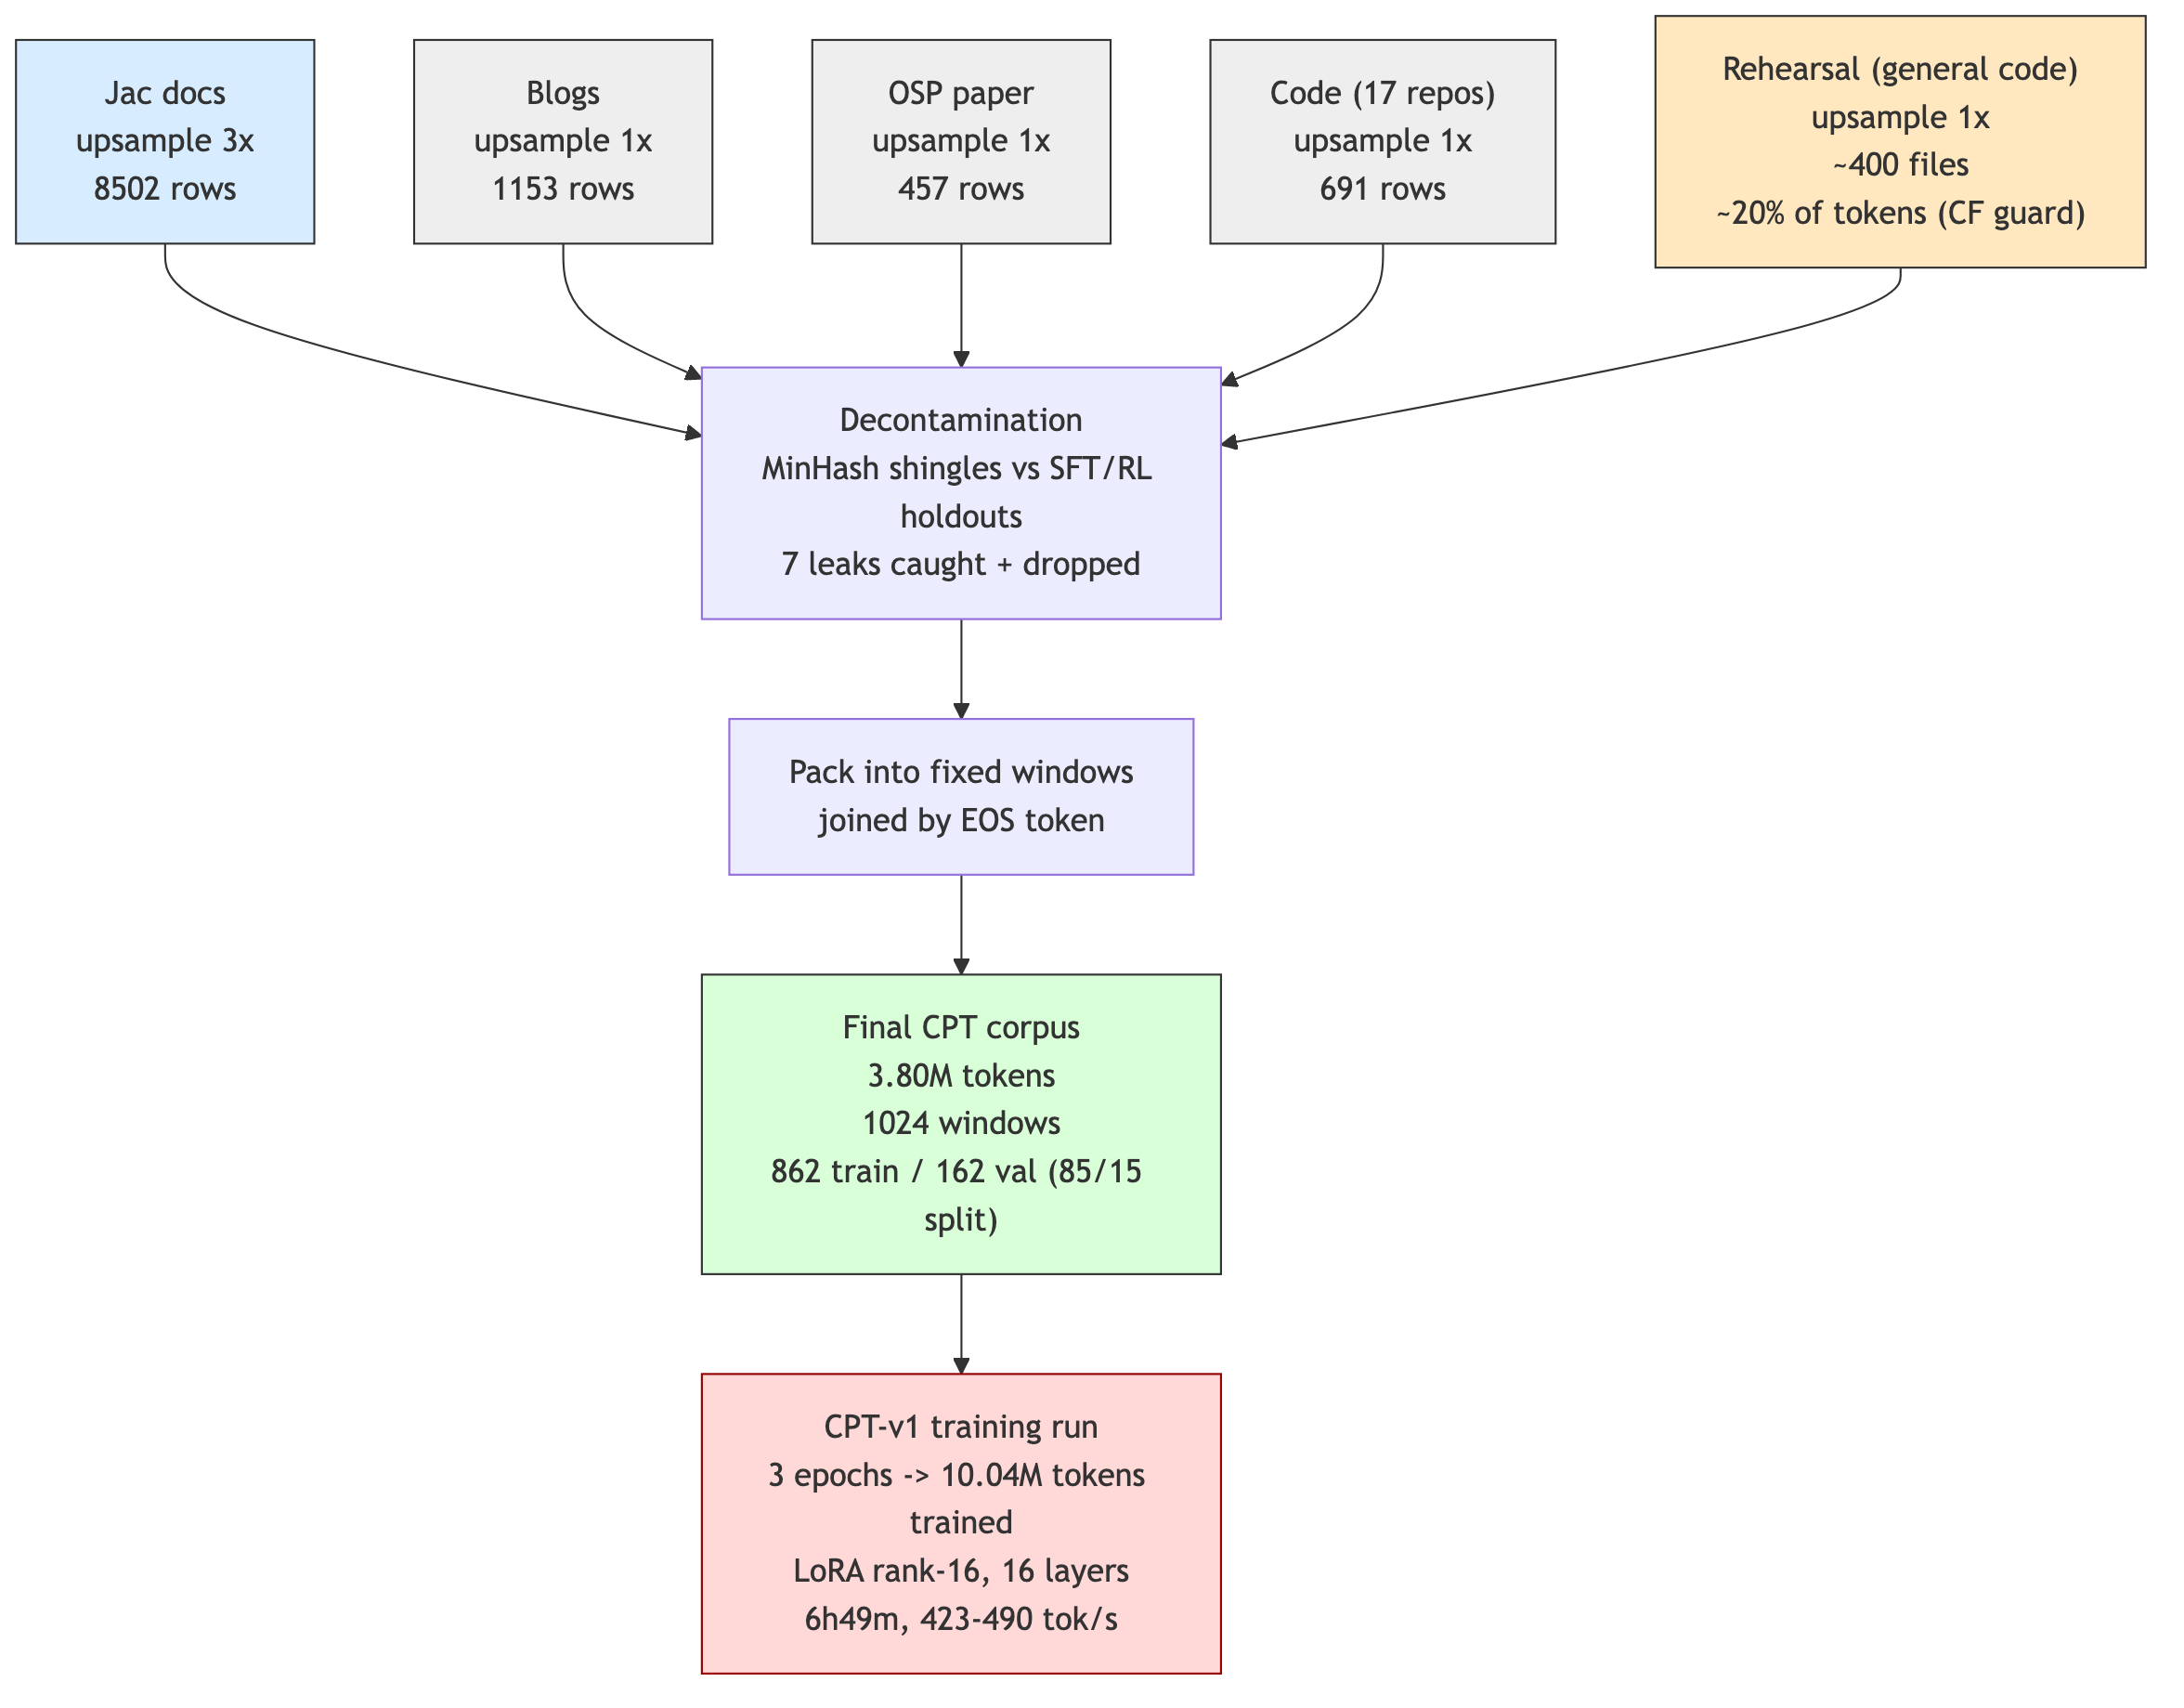
\includegraphics[width=0.85\linewidth]{dataset-diagram.png}
\end{center}

\begin{center}
\begin{tabular}{lccl}
\toprule
Source & Upsample & Rows (post-split) & Notes \\
\midrule
Jac docs & 3x & 8502 & highest quality, most curated, reinforced most \\
Blogs & 1x & 1153 & \texttt{jaseci-blogs} repo, unvetted quality \\
OSP paper & 1x & 457 & single paper, arXiv 2503.15812 LaTeX source \\
Code (org repos) & 1x & 691 & 17 Jac-bearing repos, dep-graph packed \\
Rehearsal (general code) & 1x & $\sim$400 files & CF guard, \texttt{codeparrot-clean-valid}, $\sim$20\% of tokens \\
\bottomrule
\end{tabular}
\end{center}

\textbf{Final packed size: 3.80M tokens, 1024 windows (862 train / 162 val), 85/15 split.} 3 epochs $\to$ 10.04M tokens trained.

\textbf{Decontamination}: every chunk checked against SFT/RL eval holdouts via MinHash shingles — 7 real leaks caught and dropped (holdout task mirrors inside \texttt{jac} repo examples + a shooter-demo duplicate).

\textbf{Known bug fixed pre-v1}: v1 chunker matched \texttt{\#} inside fenced code blocks as markdown headers, cutting nearly every commented code sample mid-fence. Fixed by making header detection fence-aware, then added paragraph-level splitting (docs rows 3907 $\to$ 8502). Post-fix: 9/553 (1.6\%) packed windows still start mid-sentence, all from 2 documented oversized-paragraph edge cases — not swept under the rug.

\textbf{Honest gap}: this corpus is small for real CPT (3.8M tokens vs. 100--1000x that in production runs) — the leading candidate reason for the MCQ null (see reasons slide).

\section{Slide: The two hard numbers}
\begin{center}
\begin{tabular}{lccc}
\toprule
Eval & Base (\texttt{qwen-q4}) & CPT-v1 & Delta \\
\midrule
Semantic MCQ (20 Q, greedy) & 18/20 (90\%) & 18/20 (90\%) & \textbf{0 — same 2 wrong} \\
CF regression (16 Python tasks) & 16/16 & 16/16 & 0 (no damage) \\
\bottomrule
\end{tabular}
\end{center}
CF pass = CPT didn't break general coding. MCQ null = CPT didn't teach Jac semantics either. Not noise — 20 independent questions landing on the \emph{identical} answer pattern (right and wrong) both models is a strong null, not a coin-flip artifact.

\section{Slide: What the MCQ actually asks}
20 hand-authored questions, no compiler, pure concept recognition, greedy decode (temp 0.0, deterministic). Covers: \texttt{walker} definition, \texttt{obj} vs \texttt{class}, \texttt{can...with entry}, \texttt{spawn}/\texttt{++>}, \texttt{visit}, \texttt{disengage}, \texttt{has} fields, \texttt{root}, edge filters, OSP philosophy, \texttt{by llm()}, \texttt{sem} annotations, node/edge relation, ability triggers, Jac$\leftrightarrow$Python relation, spotting a fake construct, \texttt{def} vs \texttt{can}.

\textbf{Sample question (both models got this right):}
\begin{lstlisting}
Q: What is a `walker` in Jac?
A. A traversal agent that moves through the graph, carrying
   abilities that fire at nodes/edges   <- correct
B. A static configuration file loaded at startup
C. A type of database index
D. A compiler optimization pass
\end{lstlisting}

\textbf{The 2 questions BOTH models got wrong (identical wrong answer, not just both-wrong):}

\begin{lstlisting}
Q: Which keyword does Jac prefer over `class` for defining archetypes?
A. type      <- both models answered this (WRONG)
B. obj       <- correct answer
C. struct
D. record
\end{lstlisting}

\begin{lstlisting}
Q: Which of the following is NOT a real Jac construct?
A. walker
B. spawn
C. rule (as in `rule traverse { }`)   <- correct answer
D. has       <- both models answered this (WRONG)
\end{lstlisting}

Note the irony on the second one: both models flagged \texttt{has} (a real, common keyword) as fake, while missing \texttt{rule} — the exact hallucinated construct base invented unprompted in the walker head-to-head below. Neither model reliably knows which keywords are real.

\section{Slide: Example — where CPT visibly helped (vocabulary, not correctness)}
Prompt: \emph{``Write a Jac walker named \texttt{CountNodes} that visits every node via outgoing edges and prints the count.''}

\textbf{Base (fresh) — invents a fake DSL:}
\begin{lstlisting}
walker CountNodes {
    entry = root
    rule traverse { foreach edge in self.outgoing_edges { ... } }
    continue next_node
}
\end{lstlisting}
None of \texttt{rule traverse}, \texttt{foreach edge in}, \texttt{continue next\_node} are real Jac.

\textbf{CPT-v1 — uses real Jac idiom, still not compiler-correct:}
\begin{lstlisting}
walker CountNodes {
    has root;
    has count = 0;
    rule start { spawn here -> root; }
    rule visit_node {
        self.count += 1;
        for edge in here.out_edges { spawn here -> edge.target; }
    }
}
\end{lstlisting}
\texttt{has}, \texttt{spawn}, \texttt{here.out\_edges} are genuine Jac vocabulary. \texttt{rule start} is still hallucinated. Both fail \texttt{jac check}. \textbf{Takeaway: CPT nudged style/vocabulary, not grammar} — matches design (grammar is SFT's job, not CPT's).

\clearpage
\section{Slide: The new stack (attempt 03)}
\begin{center}
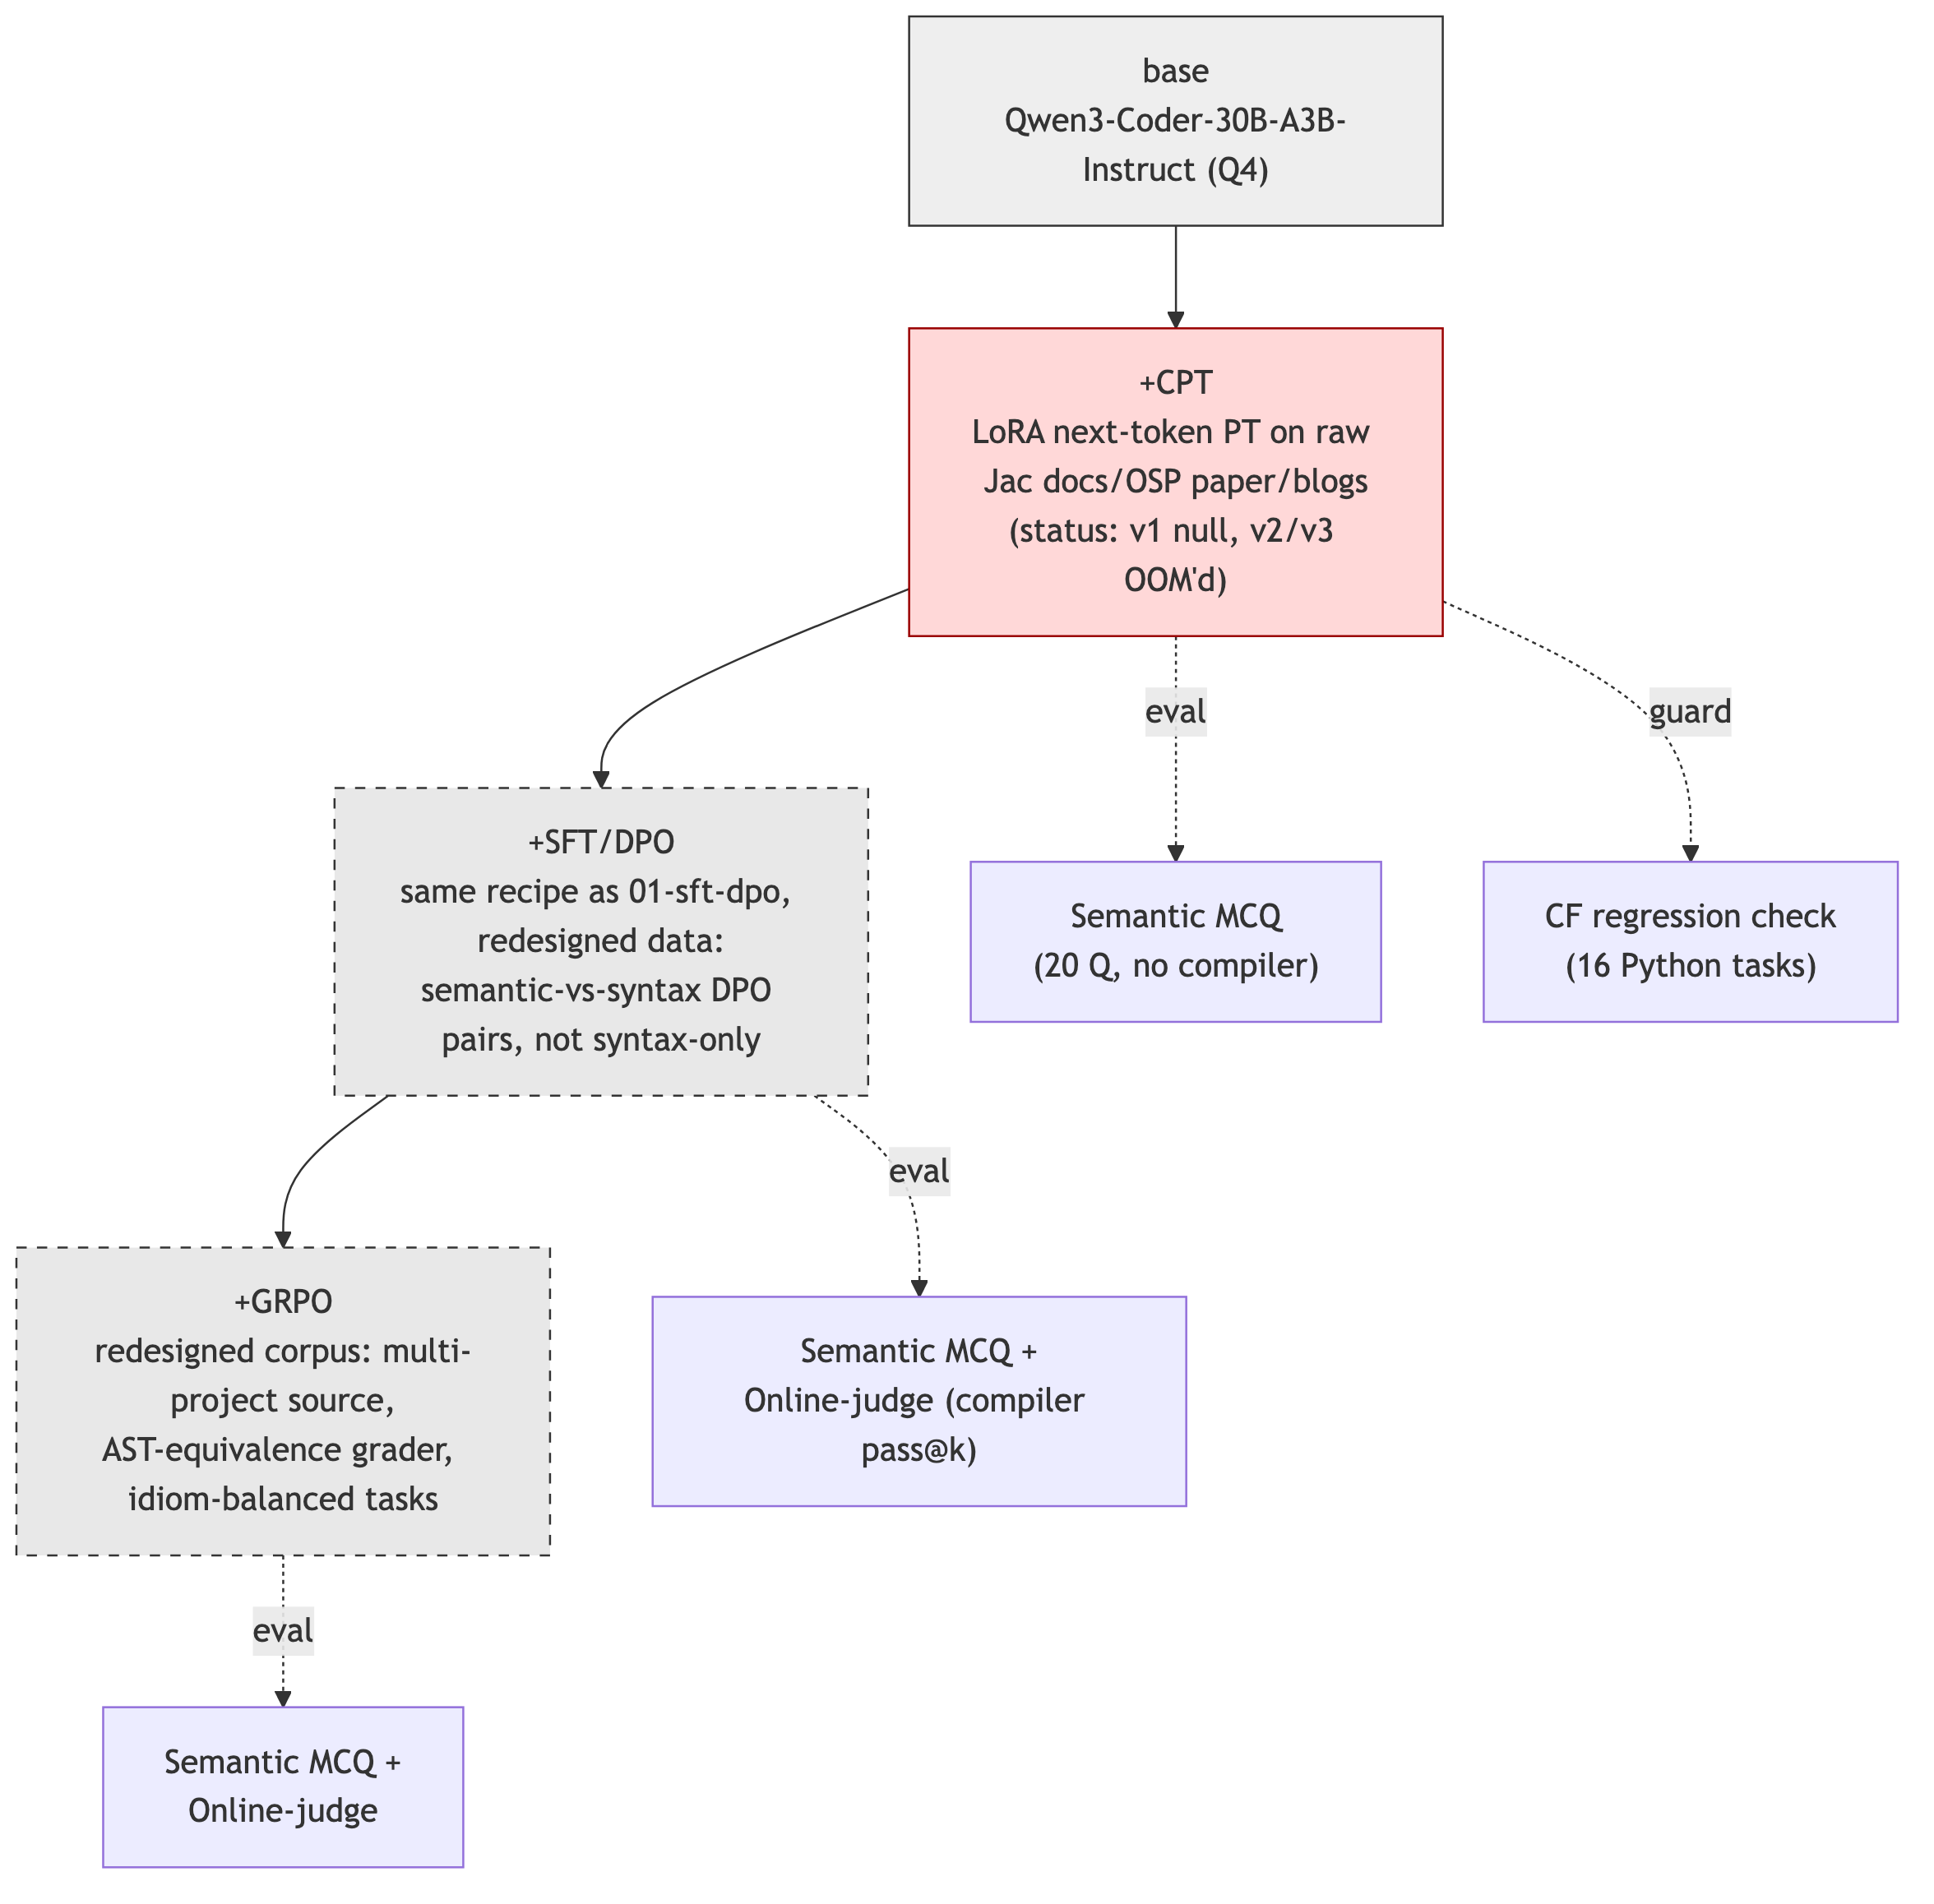
\includegraphics[width=0.95\linewidth]{stack-diagram.png}
\end{center}
4-point ablation, same base model + LoRA at every stage. CPT is the new variable this attempt adds in front of the proven \texttt{01-sft-dpo} recipe and redesigned GRPO. \textbf{Red = where we are now (CPT, null result).} Grey/dashed = not yet built — gated on CPT actually working, which it hasn't yet.

\section{Slide: Example — where CPT did NOT help (concept understanding)}
Prompt: \emph{``What's the difference between a \texttt{node} and an \texttt{edge}?''}

Both models gave near-identical answers and \textbf{both made the same wrong claim}: nodes exist at ``spatial coordinates'' / ``specific spatial locations.'' That's wrong — Jac's OSP nodes are graph-topological, not literal physical space. CPT trained directly on docs explaining this and didn't fix it. Same story on \texttt{by llm()}: both answers generic-correct, no visible improvement.

\textbf{MCQ null-result specifics (both models, same 2 wrong):}
\begin{itemize}[nosep]
  \item \texttt{obj} vs \texttt{class} keyword — both answered \texttt{type} (wrong; basic, heavily-covered fact).
  \item Which construct isn't real Jac — both picked \texttt{has} (real) instead of \texttt{rule} (the actual fabricated one, same hallucination as above).
\end{itemize}

\section{Slide: Why the null? (possible reasons)}
\begin{enumerate}
  \item \textbf{Run too small.} 3 epochs / 3.8M tokens is tiny for real CPT (production runs are 100--1000x this). Not enough exposure to shift factual recall.
  \item \textbf{LoRA capacity ceiling.} Rank-16 / 16-layer adapter may not have room to absorb new facts, only style. This project's own RL experiments hit the same kind of LoRA-scale wall before.
  \item \textbf{Wrong eval granularity, not wrong training.} Free-form generation showed a real vocabulary shift; constrained MCQ showed none. Possible CPT's effect is real but too subtle for multiple-choice to catch at this scale.
  \item \textbf{Corpus overlap with pretraining.} If base model already saw similar docs/blogs, marginal new information from a small CPT corpus is naturally low.
\end{enumerate}
Both follow-up attempts to test \#1/\#2 (v2 = 6 epochs, v3 = rank-32 full-layer) \textbf{OOM'd on 48GB unified memory before finishing} — v2 died at iter 14, v3 got to iter 100 (loss trending down, 1.5→1.16) then also OOM'd. No result either way. Hardware is the current blocker, not just data size.

\section{Recommendation slide}
\begin{enumerate}[nosep]
  \item Don't present CPT-v1 as a win. Present it as: mechanically sound, semantically null, informative negative result.
  \item Don't build next pipeline stage (SFT/DPO redesign) on top of unconfirmed CPT-v1.
  \item Fix memory footprint (smaller batch/seq len, gradient checkpointing) before re-attempting rank-32 or multi-epoch — that's the real open question, not model design.
\end{enumerate}

\end{document}
